\documentclass[10pt, conference]{IEEEtran}

\usepackage{cite}
\usepackage{url}
\usepackage{amsmath,amssymb,amsfonts}
\usepackage{algpseudocode}
\usepackage{algorithm}
\usepackage{graphicx}
\usepackage{textcomp}
\usepackage{xcolor}
\def\BibTeX{{\rm B\kern-.05em{\sc i\kern-.025em b}\kern-.08em
    T\kern-.1667em\lower.7ex\hbox{E}\kern-.125emX}}
\begin{document}

\title{Active Learning in Neural Networks\\

}

\author{\IEEEauthorblockN{DT Nicolay 26296918}
\IEEEauthorblockA{\textit{Computer Science Division} \\
\textit{Stellenbosch University}\\
Stellenbosch, South Africa \\
26296918@sun.ac.za}
}

\maketitle

\begin{abstract}
TODO
\end{abstract}

\begin{IEEEkeywords}
TODO
\end{IEEEkeywords}

\section{Introduction}
% intro

% discuss neural network

% outline of document
The theoretical background of active learning is presented in section 2, while section 3 walks through the implementation of the two active learning approaches with a neural network architecture. Section 4A describes the dataset preparation, followed by the performance criteria in section 4B. Section 4C and 4D outline the experimental design and framework for analysis. Section 5 summarises the results of the various algorithms and discusses their comparative performances with statistical analyses.

\section{Background}
The active learning paradigm and various approaches to active learning are discussed in this section. We explain how active learning is useful and how it is applied.

\subsection{Passive Learning}
% - Traditional supervised learning paradigm
% - Stochastic Gradient Descent algorithm
% - Random sampling of training data
% - Advantages and limitations
% - Mathematical formulation of SGD updates
Traditional supervised learning approaches perform passive learning during training where the algorithm has no control over which training samples it receives. That is, when techniques such as Stochastic Gradient Descent (SGD) are used, samples of the data are taken at random to update model parameters iteratively. SGD represents a form as passive learning since the model does not \textit{choose} the data points it learns from. This approach is interpretable and easy to implement, especially since there is no overhead required for observation selection.

Mathematical updates during SGD in passive learning can be expressed as:
\[
w_{t+1} = w_t - \eta \nabla_{w} L(x_i, y_i; w_t)
\]

where $\eta$ is the learning rate, $(x_i, y_i)$ is a randomly sampled observation 
from the training data at iteration $t$ and $L$ represents the loss function.



Random sampling is unbiased, but potentially inefficient in the presence of high noise and variance \cite{mahdavi}. Passive learning assumes that the distribution of the training data matches that of the test distribution, and that all the training observations contribute equally. This assumption does not always hold in practice, leading to inefficient computations. More specifically, the algorithm may waste effort on uninformative observations.


\subsection{Active Learning Paradigm}
% - Core concepts and motivation
% - Query strategy framework
% - Theoretical advantages over passive learning
In supervised learning, acquiring labeled training data for a predictive model can be very costly, but acquiring a large amount of unlabeled data is often quite easy. Active learning is a method of obtaining predictive models with high precision at a limited cost through the adaptive selection of samples for labeling \cite{Hino2020ActiveLP}. Rather than passively accepting training examples from the teacher, the network is allowed to use its current knowledge about the problem to have some deterministic control over training examples, and to guide the search for informative patterns \cite{sasla}. This may result in shorter training times due to fewer observations needing to be considered by the algorithm. That is, if the complexity of the observation selection approach does not exceed the reduction in training time achieved by considering fewer observations. Therefore, careful consideration is required to decide on an approach to observation selection.

% TODO include some math on how it may improve over passive


\subsection{Output Sensitivity Analysis}
% - Mathematical foundation of sensitivity analysis
% - How gradients indicate information content
% - Instance selection based on network sensitivity
% - Algorithm description and theoretical justification
% - Reference to SASLA.pdf concepts
For this approach, we begin by considering the entire training set and iteratively remove observations that are shown to be less informative. The neural network uses its learned knowledge of the distribution at each selection interval to do so.


% pattern informativeness
The core of this algorithm is based on pattern informativeness. The following definitions and the corresponding mathematical formulation follow the approach introduced by Engelbrecht \cite{sasla}. An informative pattern is defined as one that as a strong influence of the neural network outputs, whilst an uninformative pattern has a negligible effect. That is, the informativeness of a pattern is the sensitivity of the neural network output vector to small perturbations in the input vector. Denote the informativeness of pattern $p$ as $\Phi^{(p)}$. Then,
\begin{equation}
	\Phi^{(p)} = \lVert \mathbf{S}_o^{(p)}	 \rVert,
	\label{eq:inform}
\end{equation}

where $\mathbf{S}_o^{(p)}$ is the output sensitivity vector for pattern $p$ (defined in (\ref{eq:sens})), and $\lVert \cdot \rVert$ is any suitable norm.  
We consider the maximum-norm:

\begin{equation}
	\Phi_{\infty}^(p) = \lVert \mathbf{S}_o^{(p)} \rVert_\infty 
	= \max_{k=1,\dots,K} \{ \big| S_{o,k}^{(p)} \big| \},
	\label{eq:mn}
\end{equation}

where $S_{o,k}^{(p)}$ refers to the sensitivity of a single output unit $o_k$ to changes in the input vector $\mathbf{z}$.  

The output sensitivity vector is defined as

\begin{equation}
	\mathbf{S}_o^{(p)} = \lVert \mathbf{S}_{oz}^{(p)} \rVert,
	\label{eq:sens}
\end{equation}

where $\mathbf{S}_{oz}^{(p)}$ is the output--input layer sensitivity matrix. Assuming sigmoid activation functions in both the hidden and output layers, each element $S_{oz,ki}^{(p)}$ of the sensitivity matrix is computed as

\begin{equation}
	S_{oz,ki}^{(p)} = o_k^{(p)} \big(1 - o_k^{(p)}\big) 
	\sum_{j=1}^{J} w_{kj} \, y_j^{(p)}\big(1 - y_j^{(p)}\big) v_{ji},
\end{equation}

where $w_{kj}$ is the weight between output unit $o_k$ and hidden unit $y_j$, $v_{ji}$ is the weight between hidden unit $y_j$ and input unit $z_i$, $o_k^{(p)}$ is the activation value of output $o_k$, $y_j^{(p)}$ is the activation of hidden unit $y_j$, and $J$ is the total number of hidden units (including the bias unit to the output layer).  

Suitable norms for calculating the output sensitivity vector include the sum-norm or the Euclidean norm, i.e.,

\begin{equation}
	S_{o,k}^{(p)} = \lVert {S}_{oz}^{(p)} \rVert_1 
	= \sum_{i=1}^{I} \big| S_{oz,ki}^{(p)} \big|,
\end{equation}

or

\begin{equation}
	S_{o,k}^{(p)} = \lVert {S}_{oz}^{(p)} \rVert_2 
	= \sqrt{ \sum_{i=1}^{I} \big( S_{oz,ki}^{(p)} \big)^2 },
\end{equation}

where $I$ is the total number of input units (including the bias unit to the hidden layer).  

Using Equation~\ref{eq:mn}, a pattern is considered \textit{informative} if one or more of the output units is sensitive to small perturbations in the input vector. The larger the value of $\Phi_1^{(p)}$, the more informative the pattern $p$ is.  

To illustrate, assume gradient descent is used to find optimal weight values:

\begin{equation}
	\Delta w_{kj}, \, \Delta v_{ji} \propto \big(t_k^{(p)} - o_k^{(p)}\big),
\end{equation}

where $t_k$ is the target value for output unit $o_k$ for pattern $p$.  
Each new pattern can be viewed as a perturbation of a previously presented pattern. Let $\Phi_\infty^{(p)} = \big| S_{o,k}^{(p)}\big|$. If $\Phi_\infty^{(p)}$ is large, the output value of $o_k$ changes significantly compared to the previous presentation, making pattern $p$ highly informative. Conversely, if $\Phi_\infty^{(p)}$ is small, no significant change in $o_k$ occurs, and pattern $p$ is an insignificant contributor to the gradient direction, thus uninformative for the learning process.


\subsection{Uncertainty Sampling}
% - Uncertainty measures in classification vs regression
% - Entropy-based uncertainty for classification
% - Variance-based uncertainty for function approximation
% - Algorithm description and theoretical foundation
% - Reference to ALUS.pdf concepts
Uncertainty sampling, a frequently utilised active learning strategy, selects instances about which the model is uncertain but it does not consider the reasons for why the model is uncertain \cite{alus}. There are two reasons that a model may be uncertain about an observation. Considering a classification scenario, \textit{conflicting-evidence uncertainty} is where there is strong conflicting evidence for multiple classes. On the other hand, \textit{insufficient-evidence uncertainty} describes the situation where there is not enough evidence to classify an observation to any class. Uncertain instances often lie close to the decision boundary. Understandably, a model's variance on \textit{conflicting-evidence uncertainty} is higher than \textit{insufficient-evidence uncertainty}. 

In contrast with the output sensitivity approach, we begin with an empty set of observations and iteratively include the most uncertain observations. That is, we select an informative instance $\langle x^{*}, ? \rangle \in U$ and incorporate the new labelled instance $\langle x^{*}, y \rangle$ into $L$. More formally, Algorithm~\ref{alg:pool_active_learning} was presented by Sharma and Bilgic \cite{alus}, and describes the process of building the subset.


\begin{algorithm}
	\caption{Pool-Based Active Learning}
	\label{alg:pool_active_learning}
	\begin{algorithmic}[1]
		\State \textbf{Input:} $U$ - unlabeled data, $L$ - labeled data, $\theta$ - classification model, $B$ - budget
		\Repeat
		\For{all $\langle x^{(i)}, ? \rangle_i \in U$}
		\State compute $\text{utility}(x^{(i)}, \theta)$
		\EndFor
		\State pick highest utility $x^*$ and query its label
		\State $L \leftarrow L \cup \{\langle x^*, y^* \rangle\}$
		\State $U \leftarrow U \setminus \{\langle x^*, y^* \rangle\}$
		\State Train $\theta$ on $L$
		\State $B = B - 1$
		\Until{$B == 0$}
	\end{algorithmic}
\end{algorithm}

This study considers two ways to quantify uncertainty. First, given a probabilistic classifier that outputs a distribution over classes $P(y|x, \mathbf{w})$, the predictive entropy of an observation $x$ is defined as
\[
H(x) = - \sum_{c=1}^{C} P(y=c \mid x, \mathbf{w}) \log P(y=c \mid x, \mathbf{w}).
\]
This approach has been widely used in literature \cite{e1, e2, e3}, however often along with other techniques.

A second approach to measuring uncertainty involves using model ensembles. Instead of relying on a single model's output, construct an ensemble of models (via bootstrap sampling, random initialisations, or subspace sampling), and measure the disagreement among them. That is, for $k$ models, compute
\[
\mathrm{Var}_{k}(P(y \mid x, \mathbf{w}_k)),
\]
where $\bar P(y \mid x)$ is the mean predictive distribution across the models. Empirically, ensemble methods often provide more reliable uncertainty estimates than single-model entropy, especially in settings with model misspecification or limited data \cite{Yin2023_uncertainty_active_learning}.

\section{Implementation}

\subsection{Neural Network Architecture}
% - Single hidden layer specification
% - Hidden unit determination process (overestimate strategy)
% - Activation function selection and justification
% - Cost function selection
% - Regularisation
The neural network architecture is composed of one hidden layer, of which the number of hidden units is determined through a grid search for each problem. Figure~\ref{fig:nnarch} illustrates an overview of the architecture. Each hidden and output layer both use sigmoid activation functions. Weight decay, specifically L2 regularisation, is considered by experimenting with various penalty terms of $[0.0, 0.001, 0.01, 0.1]$ during the grid search. Momentum values of $[0.0, 0.5, 0.9, 0.95]$ are also considered during the grid search. 

\begin{figure}[htbp]
	\centering
	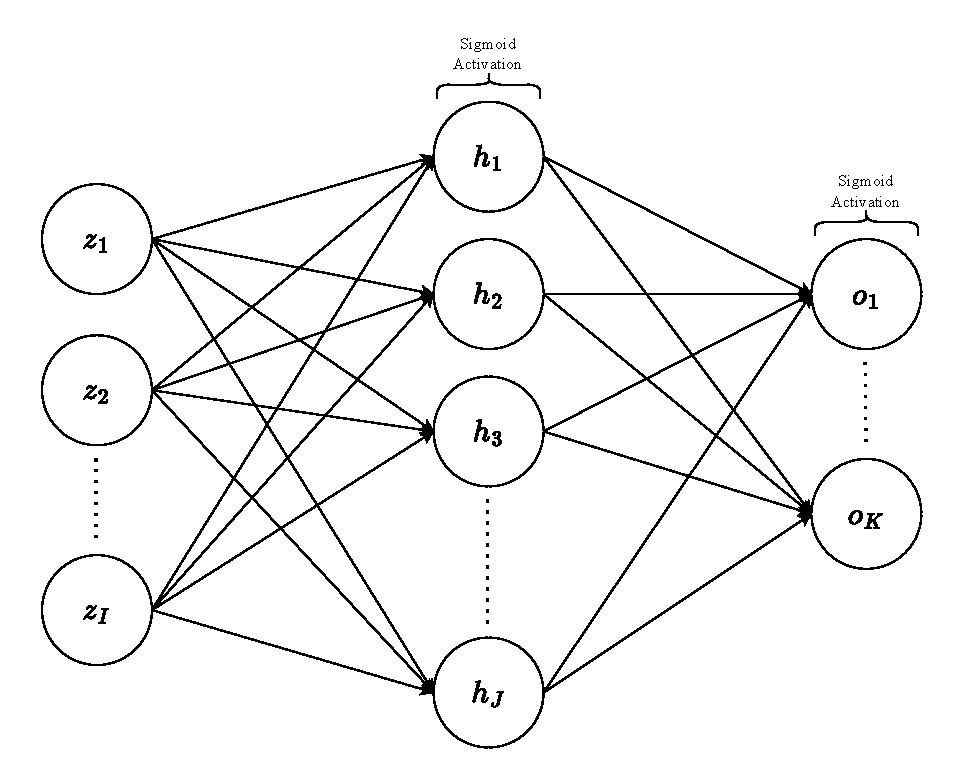
\includegraphics[width=0.45\textwidth]{images/NNarch.pdf}
	\caption{Neural network architecture. Here, $z_i$ represents input units, $h_i$ represents hidden units, and $o_i$ represents output units.}
	\label{fig:nnarch}
\end{figure}

The grid search is only performed once using the MSE Loss 
\begin{equation}
L_{\text{MSE+WD}} = \frac{1}{N} \sum_{i=1}^{N} \sum_{k=1}^{K} \big( t_{k}^{(i)} - o_{k}^{(i)} \big)^2
+\lambda \sum_{j} w_j^2
\end{equation}


\subsection{Output Sensitivity Algorithm}
% - Detailed implementation of output sensitivity analysis
% - Detailed implementation of uncertainty sampling
% - Query selection mechanisms
% - Batch size considerations for active learning

\subsection{Uncertainty Sampling Algorithm}

\subsection{Software and Hardware Specifications}
% - Programming language and libraries used
% - Computational resources
% - Code repository reference (as required)
All experiments were performed on Fedora Linux system with a 13th Gen Intel Core i3-13100 x8 CPU and 16GiB of memory. The code for this paper is available on GitHub \cite{github}.



\section{Emperical Process}
\subsection{Dataset Selection and Preprocessing}
% - Description of at least 3 classification problems
% - Description of at least 3 function approximation problems  
% - Varying complexity justification
% - Data preprocessing steps with motivations
% - Train/validation/test splits

\subsection{Performance Criteria}
% - Classification metrics: accuracy, precision, recall, F1-score
% - Function approximation metrics: MSE, MAE, R²
% - Learning curve analysis
% - Sample efficiency measures
% - Statistical significance testing approach

\subsection{Experimental Design}
% - Cross-validation strategy
% - Multiple runs for statistical reliability
% - Control parameter optimization process
% - Hyperparameter tuning methodology
% - Fair comparison ensuring protocols

\subsection{Statistical Analysis Framework}
% - Hypothesis testing approach
% - Significance levels
% - Multiple comparison corrections
% - Effect size measurements

\section{Results \& Discussion}
% (50 marks - largest section, most critical)
\subsection{Dataset Characteristics}
% - Detailed description of each dataset
% - Complexity analysis and classification difficulty
% - Baseline performance metrics

\subsection{Hyperparameter Optimization Results}
% - Optimal hidden unit numbers for each problem
% - Optimal penalty coefficients
% - Control parameter values with justifications
% - Convergence analysis

\subsection{Classification Problem Results}
% - Performance comparison across all three approaches
% - Learning curves showing sample efficiency
% - Statistical significance of differences
% - Problem-specific performance analysis
% - Tables and figures with proper captions

\subsection{Function Approximation Results}
% - Detailed results for each regression problem
% - Comparison of convergence rates
% - Sample efficiency analysis
% - Performance variance across runs

\subsection{Comparative Analysis}
% - Overall ranking of approaches
% - Problem-dependent performance patterns
% - Sample efficiency comparison
% - Computational cost analysis
% - Advantages and disadvantages of each approach

\subsection{Discussion of Findings}
% - Interpretation of results in context of theory
% - Explanation of why certain methods performed better
% - Limitations of the study
% - Practical implications for real-world applications

\section{Conclusions}
TODO

\bibliographystyle{IEEEtran}
\bibliography{references}

\end{document}
